\documentclass[11pt,fleqn]{article}
\usepackage[margin=1in]{geometry}
\usepackage{tikz}
\usepackage{mathtools}
\usepackage{longtable}
\usepackage{enumitem}
\usepackage[colorlinks = true,
		linkcolor=black,
		citecolor=black,
	        urlcolor  = black]{hyperref}
%\usepackage[dvips]{graphics}
%\usepackage[table]{xcolor}
%\usepackage{amssymb}
\usepackage{float}
%\usepackage{subfig}
\usepackage{booktabs}
\usepackage{subcaption}
\usepackage{booktabs}

\usepackage[normalem]{ulem}

\usepackage{multicol}
\usepackage{txfonts}
\usepackage{amsfonts}
\usepackage{natbib}

\usepackage{gb4e}
\usepackage[all]{xy}
\usepackage{rotating}
\usepackage{tipa}
\usepackage{multirow}
\usepackage{authblk}
\usepackage{url}
\usepackage{pdflscape}
\usepackage{rotating}
\usepackage{adjustbox}
\usepackage{array}


%\usepackage{color}
%\DeclareOuterCiteDelims{cite}{\textcolor{green}{\bibopenbracket}}{\textcolor{red}{\bibclosebracket}}

\definecolor{Pink}{RGB}{255,50,170}
\newcommand{\jd}[1]{\textcolor{Pink}{[jd: #1]}}  

\newcommand{\jt}[1]{\textbf{\color{purple}JT: #1}}

\newcommand{\tableref}[1]{Tab.~\ref{#1}}
\newcommand{\figref}[1]{Fig.~\ref{#1}}

\def\bad{{\leavevmode\llap{*}}}
\def\marginal{{\leavevmode\llap{?}}}
\def\verymarginal{{\leavevmode\llap{??}}}
\def\swmarginal{{\leavevmode\llap{4}}}
\def\infelic{{\leavevmode\llap{\#}}}

\definecolor{airforceblue}{rgb}{0.36, 0.54, 0.66}
%\definecolor{gray}{rgb}{0.36, 0.54, 0.66}

\newcommand{\dashrule}[1][black]{%
  \color{#1}\rule[\dimexpr.5ex-.2pt]{4pt}{.4pt}\xleaders\hbox{\rule{4pt}{0pt}\rule[\dimexpr.5ex-.2pt]{4pt}{.4pt}}\hfill\kern0pt%
}

\setlength{\parindent}{.3in}
\setlength{\parskip}{0ex}

\newcommand{\yi}{\'{\symbol{16}}}
\newcommand{\nasi}{\~{\symbol{16}}}
\newcommand{\hina}{h\nasi na}
\newcommand{\ina}{\nasi na}

\newcommand{\foc}{$_{\mbox{\small F}}$}

\hyphenation{par-ti-ci-pa-tion}

%\setlength{\bibhang}{0.5in}
%\setlength{\bibsep}{0mm}
%\bibpunct[:]{(}{)}{,}{a}{}{,}

\newcommand{\6}{\mbox{$[\hspace*{-.6mm}[$}} 
\newcommand{\9}{\mbox{$]\hspace*{-.6mm}]$}}
\newcommand{\sem}[2]{\6#1\9$^{#2}$}
\renewcommand{\ni}{\~{\i}}

\newcommand{\citepos}[1]{\citeauthor{#1}'s \citeyear{#1}}
\newcommand{\citeposs}[1]{\citeauthor{#1}'s}
\newcommand{\citetpos}[1]{\citeauthor{#1}'s \citeyear{#1}}

\newcolumntype{R}[2]{%
    >{\adjustbox{angle=#1,lap=\width-(#2)}\bgroup}%
    l%
    <{\egroup}%
}
\newcommand*\rot{\multicolumn{1}{R{90}{0em}}}% no optional argument here, please!

%\title{At-issueness and prior beliefs independently modulate projection}

%\thanks{For helpful comments on the research presented here, we thank the audience at the 2018 Annual Meeting of XPRAG.de and at the University of T\"ubingen. We gratefully acknowledge financial support for this research from {\em National Science Foundation} grant BCS-1452674 (JT) and the Targeted Investment for Excellence Initiative at The Ohio State University (JT). IGOR Tuebingen}}

%\author{Author(s)}

%\author[$\bullet$]{Judith Degen}
%\author[$\circ$]{Judith Tonhauser}
%
%\affil[$\bullet$]{Stanford University}
%\affil[$\circ$]{University of Stuttgart}
%
%\renewcommand\Authands{ and }

\begin{document}

\thispagestyle{empty}

\begin{center}
{\Large Prior beliefs and at-issueness independently modulate projection}

\bigskip

Word count (excluding Abstract, Supplements, and References): 2,994 words
\\ Word count (excluding Abstract and Supplements): 3,516 words
\end{center}

% Submissions should include a title page, an abstract, and should be divided into labeled sections as detailed in the style sheet.

% Glossa psycholinguistics: please add a word count (including footnotes and references) directly below the paper title. 

%The word count should not exceed ... 3,000 words for brief submissions, excluding references. 

% All references cited within the submission must be listed at the end of the main text file. Please format references and citations in APA style.

\begin{abstract}

Interpreters' inferences about what an utterance means are modulated by their \emph{prior beliefs} about contents expressed by the utterance and the extent to which such contents are \emph{at-issue} with respect to the question under discussion. %addressed by the utterance. 
Contemporary research differs with respect to whether these factors %--- prior beliefs about content and at-issueness of content --- 
are taken to independently modulate interpreters' inferences, or whether a content's at-issueness is constrained by interpreters' prior beliefs about the content. This paper reports the results of an experiment  investigating projection inferences, that is, inferences about whether the speaker is committed to content contributed by an expression in an entailment-canceling environment. The relevant expressions under investigation are sentences containing clause-embedding predicates. We replicate the effects of prior beliefs and at-issueness on projection inferences, and do not find support for the assumption that a content's at-issueness is constrained by interpreters' prior beliefs about it. This result provides support for theoretical models of utterance interpretation that assume the two factors are independent.

\vspace*{.7cm}
\noindent
{\bf Keywords:} Projection inferences; prior beliefs; at-issueness; clause-embedding predicates; English  \\

\end{abstract}

\clearpage
\pagenumbering{arabic} 

\newpage

%\begin{document}

\section{Introduction}\label{s1}

Interpreters' inferences about what an utterance means are modulated by a variety of factors. These include interpreters' prior beliefs about contents expressed by the utterance (e.g., \citealt{winograd1972,chambers-etal04,hagoort-etal2004,degen-etal2015}) and the extent to which such content is at-issue, that is, addresses the question under discussion addressed by the utterance (e.g., \citealt{Zondervan2010,degen-goodman2014,ronai2020}). One such inference are projection inferences (e.g., \citealt{langendoen-savin71,potts05}). These are inferences about the extent to which the speaker is committed to the truth of an utterance content even though that content is contributed by an expression in an entailment-canceling environment, such as polar questions. For instance, from Scott's utterance of the polar question in (\ref{first}), interpreters may infer that Scott is committed to the truth of the content of the complement of {\em discover}, that Julian dances salsa. 

\begin{exe}
\ex\label{first} Scott: ``Did Cole discover that Julian dances salsa?''
\end{exe}
Projection inferences are modulated by the question under discussion (e.g., \citealt{cummins-rohde2015,tonhauser-etal-eval}), captured by the  Gradient Projection Principle of \citet{tbd-variability}:  the extent to which content projects is positively correlated with the extent to which it is not at-issue. That is, the less Scott's utterance in (\ref{first}) is taken to address the question of whether Julian is dancing (i.e., the more that content is not at-issue), the more it projects. Projection inferences are also modulated by interpreters' prior beliefs about the content (e.g.,  \citealt{mahler2020}). For instance, the greater an interpreter's a priori belief that Julian dances salsa, the more  they take Scott to be committed to that content, that is, the more that content projects \citep{degen-tonhauser-openmind}.

Models of utterance interpretation formulated in the Rational Speech Act (RSA) framework assume that prior beliefs about and at-issueness of content independently modulate a variety of inferences, including scalar implicatures (e.g., \citealt{degen-goodman2014}). The two factors are independent in that an interpreter's prior beliefs about content are modeled as affecting interpretation directly, whereas the at-issueness of content is modeled as affecting the speaker's production model and therefore only entering interpretation indirectly, via consideration of the speaker model. And, indeed, extant RSA models of projection inferences implicitly assume that the two factors are independent, as they assume uniform priors but changing questions under discussion (\citealt*{qing-etal2016,stevens-etal2017}). In contrast, the two factors are not independent according to the Non-redundancy Principle for At-issue Content \citep*{tonhauser-etal-eval}: according to this principle, the more an interpreter takes a content to be a priori true (i.e., before observing an utterance), the less likely it is that they take the speaker to have intended for the content to be at-issue with respect to the implicit question under discussion.

This paper reports on the results of an experiment designed to investigate whether prior beliefs about and at-issueness of a content independently modulate its projection, as assumed in RSA models, or whether the two factors interact, as hypothesized in \citealt{tonhauser-etal-eval}. The particular type of content whose projection is investigated is the content of the complement of English clause-embedding predicates, like {\em discover} in (\ref{first}). Projection research has long recognized that predicate meaning modulates the projection of the content of the clausal complement, such that, for instance, content embedded under {\em discover} is less projective than content embedded under {\em know} (e.g., \citealt{kiparsky-kiparsky70,degen-tonhauser-language}). The experiment therefore includes the meaning of the clause-embedding predicate as a third factor that modulates projection. RSA models lead us to expect that prior beliefs modulate projection inferences independently of the predicate, whereas the at-issueness of content should interact with the predicate, as both affect the speaker's production model.

\section{Experiment}\label{s2}

The experiment investigates the relation between interpreters' prior beliefs about content and the content's at-issueness in modulating its projection. Participants rated the prior probability, at-issueness, and projection of 20 contents. %At-issueness was measured using the `asking-whether' diagnostic used by \citet{tbd-variability}. The target items and measures of the prior beliefs and projection were identical to those used by \citet{degen-tonhauser-openmind}. % Exps.~1 and 2, and \citepos{degen-tonhauser-language} Exp.~1a. 

\subsection{Methods} 
 
\paragraph{Participants} 600 participants with U.S.\ IP addresses and at least 99\% of previous HITs approved were recruited on Amazon's Mechanical Turk platform (ages: 18-73, median: 38.5). They were paid \$2.20.

\paragraph{Materials and procedure} The prior probability, at-issueness, and projection of the contents of 20 clauses were measured in three separate blocks. Prior probability was manipulated by pairing each of the 20 clauses (e.g., \emph{Julian dances salsa})  with two facts between participants: the content of each clause was expected to have a higher prior probability in the presence of one fact (e.g., \emph{Julian is Cuban}) than of the other (e.g., \emph{Julian is German}). See Supplement \ref{a-stim} for the full set of 20 clauses and facts, and Supplement \ref{a-beliefs} for evidence that the facts successfully manipulated the prior probability of the respective contents.

In the prior block, the 20 clauses were realized as the complements of {\em How likely is it that\ldots?}~questions \citep{degen-tonhauser-openmind}. As shown in Fig.~\ref{fig-exp1-prior}, each target item consisted of one of the two facts for that clause and the {\em How likely is it that\ldots?} question. Participants read the fact and assessed the prior probability of the content, given the fact. They gave their responses on a slider marked `impossible' at one end (coded as 0) and `definitely' at the other (coded as 1). 

In the at-issueness and projection blocks, target items consisted of a fact and a polar question that was uttered by a named speaker, as in Fig.~\ref{fig-exp1-nai} and Fig.~\ref{fig-exp1-projection}, respectively. The polar questions were formed by realizing the 20 clauses as the complements of the 20 clause-embedding predicates  in Fig.~\ref{fig-exp1-predicates}. Participants were told to imagine that they are at a party and that, on walking into the kitchen, they overhear somebody ask somebody else a question. At-issueness was measured using the `asking whether' diagnostic (\citealt{tbd-variability}): participants were asked to rate whether the speaker was asking about the content of the complement (CC), taking into consideration the fact. They gave their responses on a slider marked `yes' at one end (coded as 0) and `no' at the other (coded as 1). Greater not-at-issueness of the CC with respect to the implicit question under discussion should result in higher slider ratings. Projection was measured using the `certain that' diagnostic (\citealt{tbd-variability, mahler2020}): participants were asked to rate whether the speaker was certain of the CC, taking into consideration the fact. They gave their responses on a slider marked `no' at one end (coded as 0) and `yes' at the other (coded as 1). Greater projection of the CC should result in higher slider ratings. 

\begin{figure}[h!]
\centering

\begin{subfigure}[t]{0.5\textwidth}
        \centering
\fbox{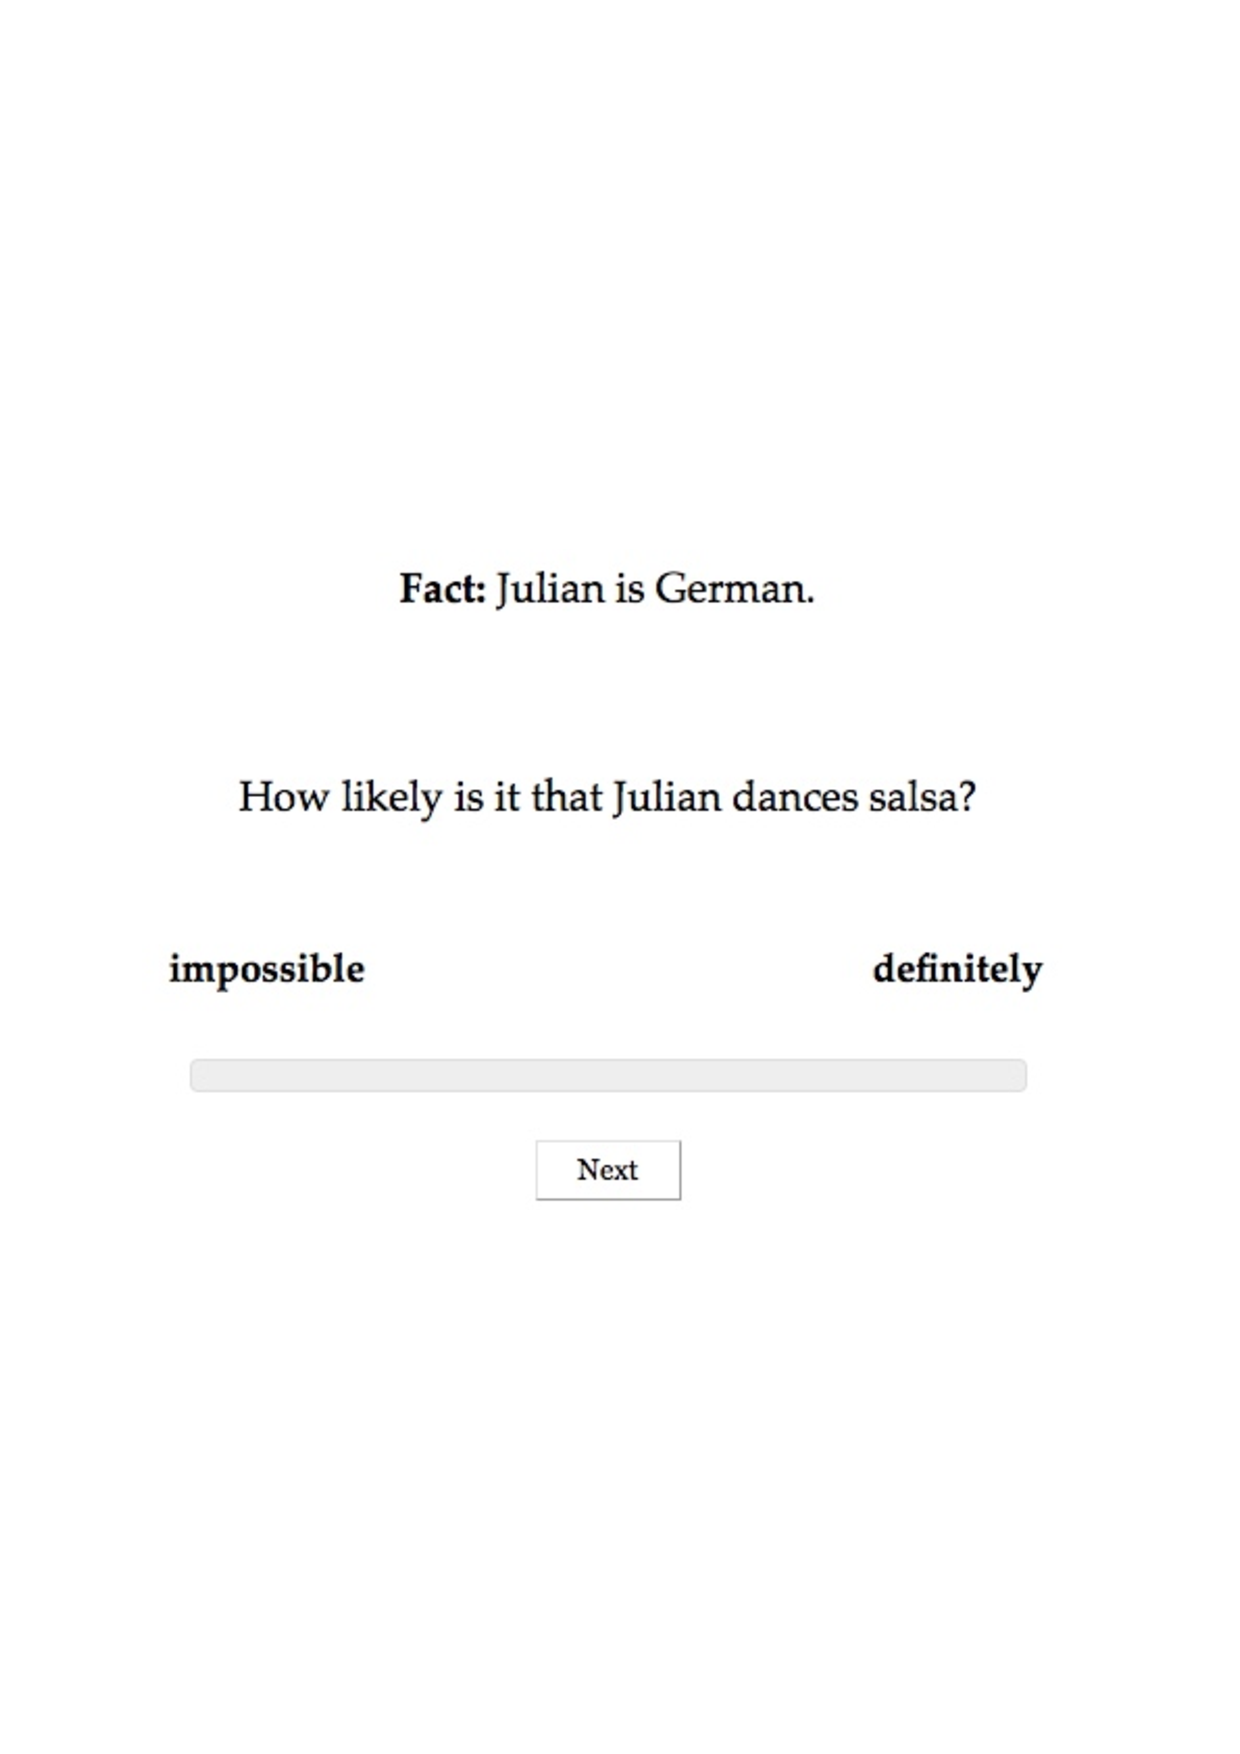
\includegraphics[width=7.6cm]{figures/exp1-prior-trial}}
\caption{Target trial in prior block.}\label{fig-exp1-prior}
\end{subfigure}
 \par\bigskip
\begin{subfigure}[t]{0.8\textwidth}
\par\bigskip
\centering
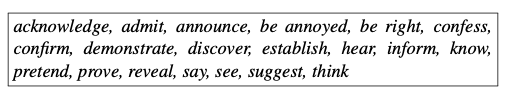
\includegraphics[width=10cm]{figures/predicates}
\caption{20 clause-embedding predicates in not-at-issueness and projection blocks.}\label{fig-exp1-predicates}
 \end{subfigure}
 \par\bigskip
\begin{subfigure}[t]{0.5\textwidth}
\par\bigskip
\centering
 \fbox{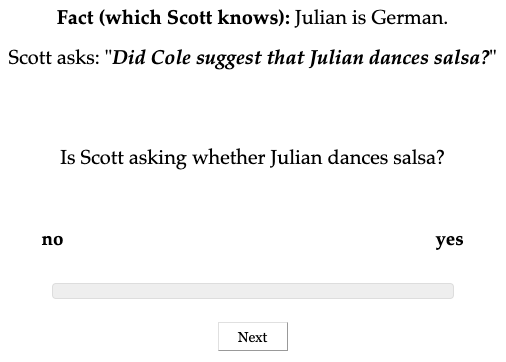
\includegraphics[width=7.6cm]{figures/exp1-nai-trial}} 
\caption{Target trial in not-at-issueness block.}\label{fig-exp1-nai}
 \end{subfigure}%
 \begin{subfigure}[t]{0.5\textwidth}
\par\bigskip
\centering
 \fbox{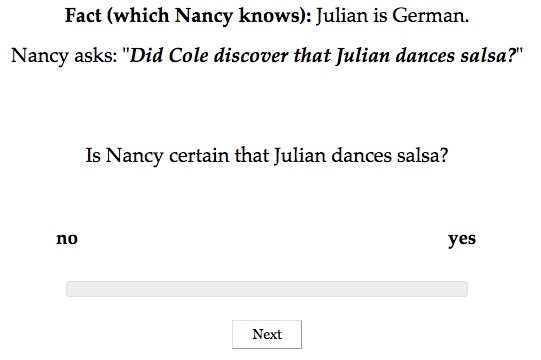
\includegraphics[width=7.6cm]{figures/exp1-projection-trial}} 
\caption{Target trial in projection block.}\label{fig-exp1-projection}
 \end{subfigure}

\caption{Sample target trials and clause-embedding predicates in the experiment.}
\end{figure}

The at-issueness and projection blocks also included 6 control trials each, which functioned as attention checks: the contents of these items were expected to be at-issue and not to project. The same 6 contents were also used to form 6 filler trials in the prior block. These filler items were not used to assess participants' attention. For the full set of control and filler items see Supplement \ref{a-stim}.

Each participant's set of items was semi-randomly generated: first, the 20 clauses were randomly paired with the 20 predicates. Then, one random half of the items was assigned the respective clause's higher-probability fact, and the other half its lower-probability fact. Participants completed a total of 78 trials: 20 target trials in each block, 6 control trials in the projection and at-issueness blocks each, and 6 filler trials in the prior block. Each participant completed the same filler and control trials. The prior block was presented first to all participants; the projection and at-issueness blocks were then presented in random order. Within blocks, trial order was randomized.

After completing the experiment, participants filled out a short optional demographic survey. To encourage truthful responses, participants were told that they would be paid no matter what answers they gave in the survey.

\paragraph{Data exclusion} Data was excluded based on self-declared non-native speaker status and other criteria shown in Supplement \ref{a-excl}, leaving 10,100 data points from 505 participants (ages 20-73; mean age: 39.5).

\subsection{Results}

Fig.~\ref{fig:certainty-by-prior} shows participants' certainty ratings (measuring projection) against prior probability ratings: the positive correlation suggests that the higher an interpreter's prior belief about content is, the more that content projects, as also observed in \citealt{degen-tonhauser-openmind}. Fig.~\ref{fig:certainty-by-nai} shows participants' certainty ratings (measuring projection) against asking-whether ratings (measuring not-at-issueness): the positive correlation suggests the more a content is not-at-issue, the more that content projects, as predicted by \citepos{tbd-variability} Gradient Projection Principle. In contrast, Fig.~\ref{fig:prior-by-nai}, which shows participants' asking-whether ratings (measuring not-at-issueness) against prior probability ratings, suggests that a content's not-at-issueness is independent of interpreters' prior beliefs about the content, contrary to \citepos{tonhauser-etal-eval} Non-redundancy Principle for At-issue Content.

\begin{figure}[h!]
\centering
\begin{subfigure}[t]{0.33\textwidth}
%\par\bigskip
%\centering
\includegraphics[width=\textwidth]{../results/main/exp3/graphs/Fig2a-certainty-by-prior}
\caption{}\label{fig:certainty-by-prior}
\end{subfigure} \hfill
\begin{subfigure}[t]{0.33\textwidth}
%\par\bigskip
%\centering
\includegraphics[width=\textwidth]{../results/main/exp3/graphs/Fig2b-certainty-by-nai}
\caption{}\label{fig:certainty-by-nai}
 \end{subfigure}\hfill
 \begin{subfigure}[t]{0.33\textwidth}
%\centering
\includegraphics[width=\textwidth]{../results/main/exp3/graphs/Fig2c-nai-by-prior}
\caption{}\label{fig:prior-by-nai}
\end{subfigure} 
\caption{Participants' (a) certainty ratings against prior probability ratings,  (b) certainty ratings against asking-whether ratings, and (c) prior probability ratings against asking-whether ratings. Linear smoothers with 95\% confidence intervals overlaid.}\label{fig:results}
\end{figure}

%cprior                  0.16115    0.01146  385.42598  14.057  < 2e-16 ***
%not-at-issue $^*$                     0.19776    0.01486  571.38803  13.311  < 2e-16 ***
%cblock_ai               0.03539    0.01211  468.54516   2.923  0.00364 ** 
%prior prob. $^*$ not-at-issue $^*$              0.02951    0.02285 3481.97261   1.291  0.19664 
%prior prob. $^*$ cblock_ai        0.08649    0.02231  500.58065   3.877  0.00012 ***
%not-at-issue $^*$cblock_ai          -0.04754    0.02260  436.29891  -2.103  0.03602 *  
%prior prob. $^*$ not-at-issue $^*$cblock_ai   -0.02684    0.04483 6871.98493  -0.599  0.54932

These observations were borne out statistically.\footnote{All analyses were conducted in R (\citealt{R}, version 4.1.2) using the {\tt lme4} package (\citealt{bates-etal2015}). P-values were obtained via Satterthwaite approximations as implemented in the {\tt lmerTest} package (\citealt{kuznetsova-etal2017}).}  To assess whether at-issueness  and prior beliefs  modulate projection, we fit a mixed-effects linear regression predicting certainty ratings from a centered fixed effect of asking-whether rating, a centered fixed effect of prior probability rating, a centered fixed effect of block (with `at-issueness as 2nd block' as the reference level before centering), and their interactions. The model included the maximal random effects structure justified by the data and the theoretical assumptions: random by-item and by-participant intercepts,\footnote{An item is a combination of a predicate and an embedded clause.} and random by-item and by-participant slopes for the prior probability and asking-whether fixed effects. There were significant main effects of  asking-whether rating ($\beta$ = .2,  $SE$ = .01, $t$=13.3, $p<$ .001) and prior probability rating ($\beta$ = .16,  $SE$ = .01, $t$=14.1, $p<$ .001)  on certainty ratings in the expected direction.\footnote{There was also a significant main effect of block ($\beta$ = .04,  $SE$ = .01, $t$=2.9, $p<$ .01), such that certainty ratings were higher when the projection block immediately followed the prior block, as well as a significant interaction of prior probability ratings and block ($\beta$ = .09,  $SE$ = .02, $t$=3.9, $p<$ .001), and  of asking-whether and block ($\beta$ = -.05,  $SE$ = .02, $t$=-2.1, $p<$ .05). This suggests that the effect of prior beliefs and at-issueness on projection was stronger when the corresponding block immediately preceded the projection block. The three-way interaction was not significant.} These results replicate \citepos{degen-tonhauser-openmind} result -- that prior beliefs modulates projection -- and they are consistent with \citepos{tbd-variability} Gradient Projection Principle --- that at-issueness modulates projection. Critically, the interaction between prior probability and asking-whether ratings was not significant ($\beta$ = .03,  $SE$ = .02, $t$=1.3, $p=$ .2). While null effects should be interpreted with caution, this preliminarily suggests that prior probability and at-issueness independently modulate projection. 

%cprior      3.927e-03  1.161e-02 3.320e+02   0.338    0.735 
To further investigate the relation between at-issueness and prior beliefs, we fit a mixed-effects linear regression predicting asking-whether ratings from a centered fixed effect of prior probability rating.\footnote{Fixed effects of block and its interaction with prior probability ratings did not reach significance and were therefore omitted from the model reported here.} The model included random by-item and by-participant intercepts, and random by-item and by-participant slopes for prior probability. There was no main effect of prior probability rating ($\beta$ = .004,  $SE$ = .01, $t$=.3, $p=$ .7), further suggesting that the at-issueness of and prior beliefs about content are independent of each other. This result supports an assumption made by RSA models: that interpreters' prior beliefs about utterance content and the at-issueness of utterance content independently modulate projection inferences, contrary to the interaction hypothesized in \citealt{tonhauser-etal-eval}.

We next examined the interaction between the two factors and predicate meaning. Fig.~\ref{fig:results2} shows participants' certainty ratings against prior probability ratings (panel a) and asking-whether ratings (panel b) by clause-embedding predicate; the predicates are ordered by the strength of the projection of the content of their complements (least projective: {\em pretend}; most projective: {\em be annoyed}).\footnote{Our experiment replicates the result from \citepos{degen-tonhauser-language} Exp.~1a and \citepos{degen-tonhauser-openmind} Exp.~1 that predicate meaning modulates the projection of the content of the clausal complement (Spearman rank correlations: .982 and .985; for visualizations see Supplement \ref{a-replication}). } The positive correlations in Fig.~\ref{fig:certainty-by-prior-and-predicate} suggest that the effect of prior probability on projection is independent of predicate meaning. By contrast,  Fig.~\ref{fig:certainty-by-nai-and-predicate} suggests an interaction between at-issueness and predicate meaning: whereas there is a positive correlation for most predicates, some display none or a negative one. %, including {\em be right}, a negative or zero correlation is observed for predicates like {\em pretend} or {\em prove}, respectively.

\begin{figure}[h!]
\centering
\begin{subfigure}[t]{0.5\textwidth}
\par\bigskip
\centering
\includegraphics[width=\textwidth]{../results/main/exp3/graphs/Fig3a-certainty-by-prior-and-predicate}
\caption{Certainty against prior probability ratings.}\label{fig:certainty-by-prior-and-predicate}
\end{subfigure}%
\begin{subfigure}[t]{0.5\textwidth}
\par\bigskip
\centering
\includegraphics[width=\textwidth]{../results/main/exp3/graphs/Fig3b-certainty-by-nai-and-predicate}
\caption{Certainty against asking-whether ratings.}\label{fig:certainty-by-nai-and-predicate}
 \end{subfigure}


\caption{Certainty ratings against (a) prior probability ratings and (b) asking-whether ratings, by predicate. Linear smoothers with 95\% confidence intervals overlaid.}\label{fig:results2}
\end{figure}


These observations were confirmed by mixed-effects linear regression models predicting certainty ratings from a centered fixed effect of prior probability or asking-whether rating, predicate,\footnote{To facilitate the interpretation of the interactions, the reference level was set to the predicate for which the slope of the fixed effect on certainty rating was closest to 0, namely {\em be annoyed} (fixed effect: prior probability) and {\em prove} (fixed effect: asking-whether).} and their interaction. The models included the maximal random effects structure that was justified by the design and that allowed them to converge: random by-clause and by-participant intercepts, and random by-clause and by-participant slopes for the prior probability or asking-whether fixed effects, respectively. The positive effect of prior probability on certainty ratings was observed for the contents of the complements of all predicates, suggesting that prior beliefs modulate projection across predicates. This result replicates \citealt{degen-tonhauser-openmind}. 

There was a significant effect of asking-whether on certainty ratings for most of the predicates, but not for {\em confirm, demonstrate, establish, prove} and {\em say}, and a negative effect for {\em pretend, suggest}, and {\em think}. (See Supplement \ref{a-models} for model details.) This result suggests that projection inferences are not consistently modulated by the question under discussion.

\section{General discussion and concluding remarks}\label{s-disc}

Prior research suggests that projection inferences, that is, inferences about the extent to which the speaker is committed to the truth of non-entailed content, are modulated both by interpreters' prior beliefs about the content (\citealt{degen-tonhauser-openmind}) and the content's at-issueness with respect to the question under discussion (\citealt{tbd-variability}). The main result of the experiment reported on in this paper suggests that these two factors independently modulate projection inferences, rather than at-issueness being constrained by, or even reducible to, interpreters' prior beliefs about the content (cf.\ \citealt{tonhauser-etal-eval}). 

This result provides empirical support for formal models of projection inferences that acknowledge the independent contribution of these two factors, such as the RSA models presented in \citealt{qing-etal2016} and \citealt{stevens-etal2017}. Unfortunately, neither of these models naturally extend to the projection inferences investigated in this paper. \citepos{qing-etal2016} analysis is limited to projection inferences that are triggered by change-of-state verbs like \emph{stop}, whereas the inferences investigated here arise from a wide variety of clause-embedding predicates, albeit to varying degrees. \citepos{stevens-etal2017} analysis is designed for projection inferences triggered by utterances' prosody. Even though the projection inferences investigated here are also modulated by prosody (see, e.g., \citealt{tonhauser-salt26,djaerv-bacovcin-salt27}), an empirically adequate analysis must also capture the variable contributions of the lexical meanings of the clause-embedding predicates to projection inferences. Developing such an analysis is a pressing task for future research.

Finally, our experiment revealed that a content's at-issueness with respect to the question under discussion does not invariably modulate projection of the content. Rather, our experiment revealed an interaction between the question under discussion and the meaning of the predicate that embeds the content. A predictive model of projection inferences must include a systematic account of this interaction. We hypothesize that (yet to be identified) components of lexical meaning constrain whether the projection of the content of the clausal complement is modulated by the question under discussion. For instance, an analysis according to which the lexical meaning of {\em pretend} entails that the speaker is committed to the falsity of the content of the complement predicts that this content does not project even when it is not at-issue. %(it does not yet, however, predict the observed negative correlation).
Which components of lexical meaning play a role in modulating projection inferences is an important question for future research. 

%\jd{why an overridable default and not the opposite: a principle that can only be applied under certain lexical semantic circumstances? i'm generally not a huge fan of defaults, because they tend to be arbitrary. not sure yet how best to put this, because the main point is: we need a predictive model of projection inferences that includes the interaction of lexical semantics and qud in a systematic way, and that allows us to pinpoint, e.g.: if the lexical semantics includes feature X, then the qud is irrelevant (i.e., has no power to modulate projection). if the lexical semantics includes feature Y, then the qud has space to do (more or less) work.}

\section*{Data accessibility statement}

The experiment, data, and R code for generating the figures and analyses reported on in this paper are available at [link redacted for review]
%\href{https://github.com/judith-tonhauser/attitude\_preds\_projection}{https://github.com/judith-tonhauser/attitude\_preds\_projection}
. The experiment was preregistered at [link redacted for review].
%\href{https://osf.io/tg2bn}{https://osf.io/tg2bn}.

\section*{Ethics and consent}

The experiment was declared exempt from review by the IRB of [university redacted for review]. Informed consent was obtained from the participants.

%\section*{Acknowledgments}
%(removed for review)

\bibliographystyle{cslipubs-natbib}
%\bibliographystyle{apacite}
\bibliography{bibliography}

% uncomment for word count
%\end{document}

\newpage

\appendix

\setcounter{table}{0}
\renewcommand{\thetable}{A\arabic{table}}

\setcounter{figure}{0}
\renewcommand{\thefigure}{A\arabic{figure}}

\section*{Supplements}

\section{Target and control items}\label{a-stim}

\paragraph{Target items} This list shows the 20 clauses of the target items alongside their lower and higher probability facts, respectively:

\begin{enumerate}[leftmargin=4ex,itemsep=-2pt]
\item Mary is pregnant. Facts: Mary is a middle school student / Mary is taking a prenatal yoga class
\item Josie went on vacation to France. Facts:  Josie doesn't have a passport / Josie loves France 
\item Emma studied on Saturday morning. Facts: Emma is in first grade / Emma is in law school 
\item Olivia sleeps until noon. Facts: Olivia has two small children / Olivia works the third shift
\item Sophia got a tattoo. Facts: Sophia is a high end fashion model / Sophia is a hipster
\item Mia drank 2 cocktails last night. Facts: Mia is a nun / Mia is a college student
\item Isabella ate a steak on Sunday. Facts: Isabella is a vegetarian / Isabella is from Argentina
\item Emily bought a car yesterday. Facts: Emily never has any money / Emily has been saving for a year
\item Grace visited her sister. Facts: Grace hates her sister / Grace loves her sister
\item Zoe calculated the tip. Facts: Zoe is 5 years old / Zoe is a math major
\item Danny ate the last cupcake. Facts: Danny is a diabetic / Danny loves cake
\item Frank got a cat. Facts: Frank is allergic to cats / Frank has always wanted a pet
\item Jackson ran 10 miles. Facts: Jackson is obese / Jackson is training for a marathon
\item Jayden rented a car. Facts: Jayden doesn't have a driver's license / Jayden's car is in the shop
\item Tony had a drink last night. Facts: Tony has been sober for 20 years / Tony really likes to party with his friends
\item Josh learned to ride a bike yesterday. Facts: Josh is a 75-year old man / Josh is a 5-year old boy
\item Owen shoveled snow last winter. Facts: Owen lives in New Orleans / Owen lives in Chicago
\item Julian dances salsa. Facts: Julian is German / Julian is Cuban
\item Jon walks to work. Facts: Jon lives 10 miles away from work / Jon lives 2 blocks away from work
\item Charley speaks Spanish. Facts: Charley lives in Korea / Charley lives in Mexico
\end{enumerate}

In the target items of the projection and at-issueness blocks, eventive predicates, like {\em discover} and {\em hear}, were realized in the past tense and stative predicates, like {\em know} and {\em be annoyed}, were realized in the present tense. The direct object of {\em inform} was realized by the proper name {\em Sam}. Each clause-embedding predicate was paired with a unique subject proper name. The speaker of the target items was realized by a randomly sampled unique proper name. 

\paragraph{Control and filler items} The not-at-issueness and projection blocks included 6 control trials each; sample control trials are shown in Fig.~\ref{fig-exp1-nai-control} and Fig.~\ref{fig-exp1-projection-control}, respectively. The full set of control items is given in (\ref{control-items}). The content of these items was expected to be at-issue and not to project: For example,  in Fig.~\ref{fig-exp1-nai-control}, the speaker is asking about the main clause content, that is, whether Samantha has a new hat, and, in Fig.~\ref{fig-exp1-projection-control}, the speaker is not committed to the main clause content, that Samantha has a new hat. The same 6 main clauses were also used to form 6 filler trials in the prior block; a sample trial is given in Fig.~\ref{fig-exp1-prior-filler}. These filler items were not used to assess participants' attention. 

\begin{figure}[h!]
\centering
\begin{subfigure}[t]{0.5\textwidth}
        \centering
\fbox{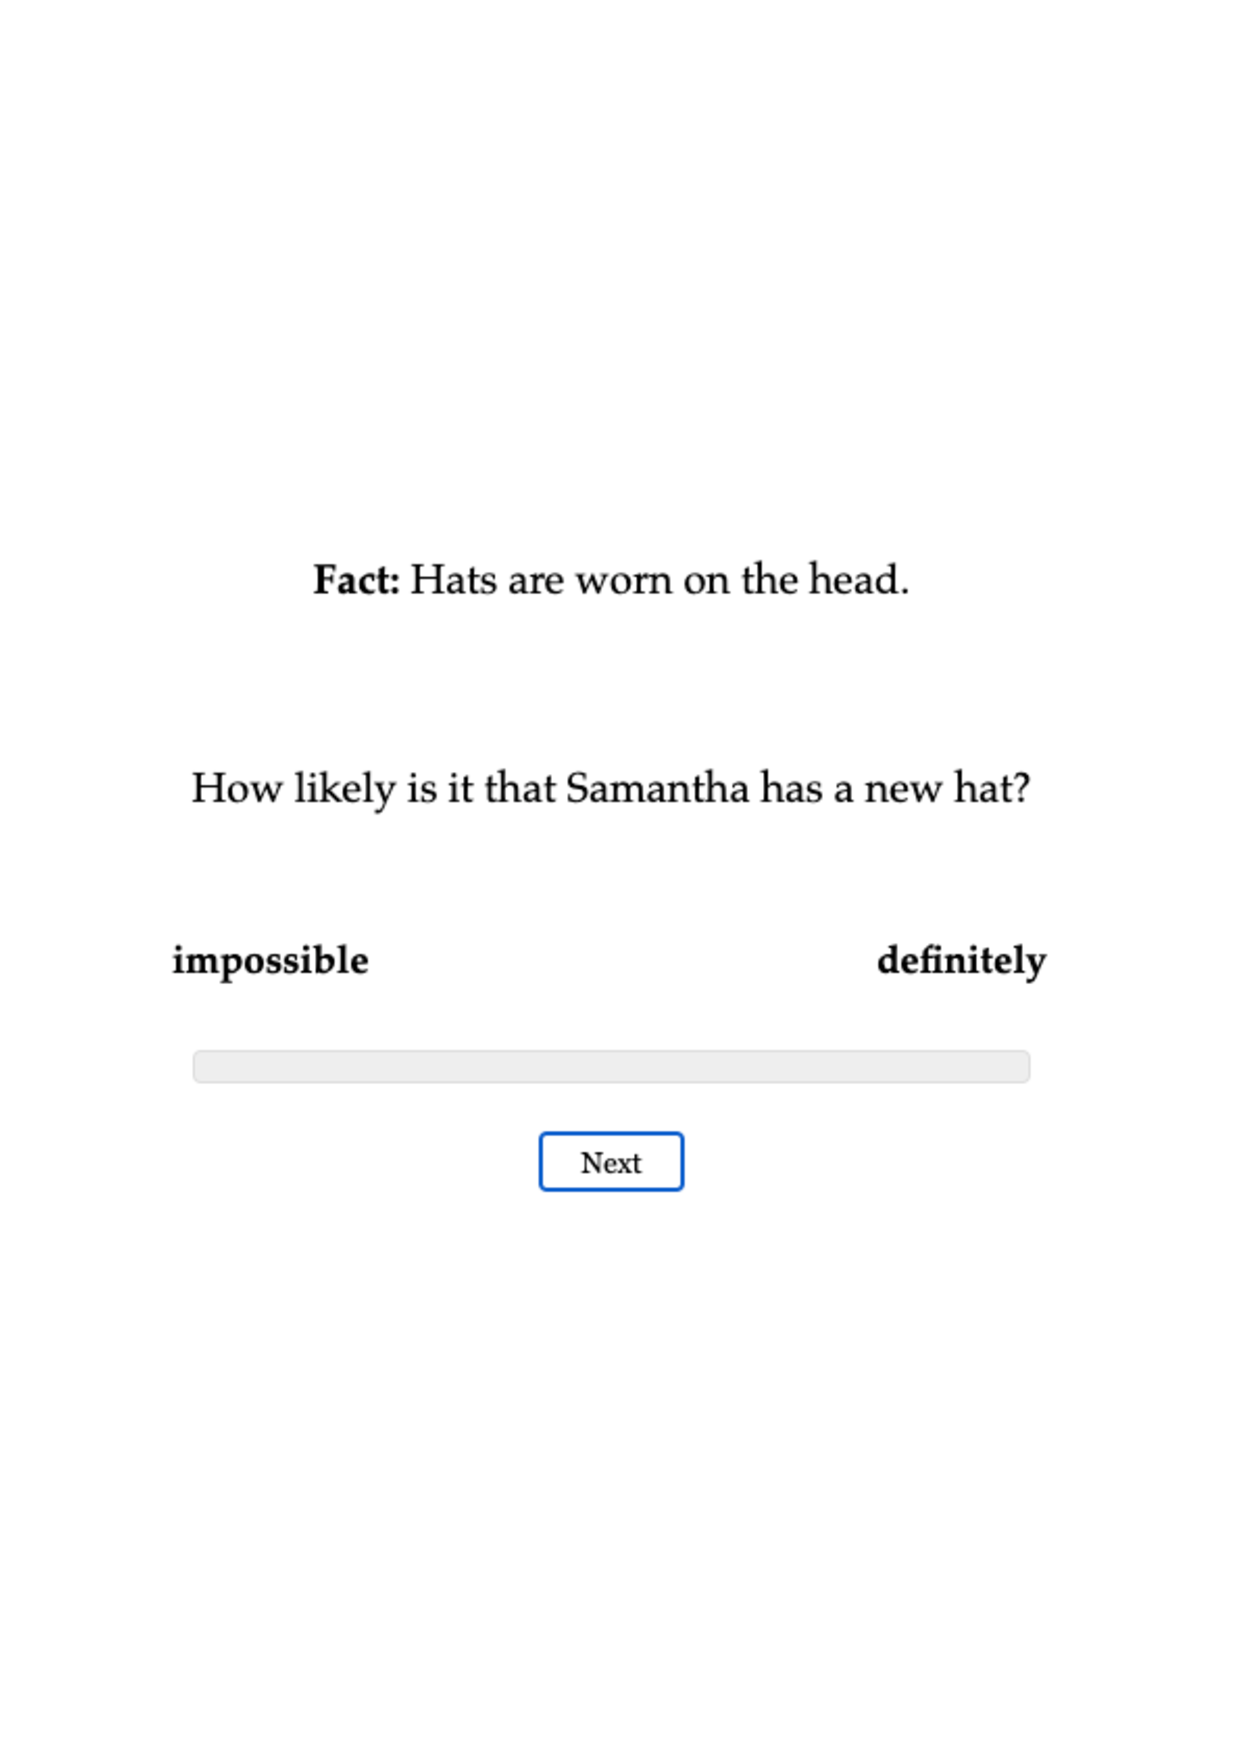
\includegraphics[height=5.4cm,width=7.6cm]{figures/exp1-prior-filler}}
\caption{Filler trial in prior block.}\label{fig-exp1-prior-filler}
 \end{subfigure}
\begin{subfigure}[t]{0.5\textwidth}
\centering
\fbox{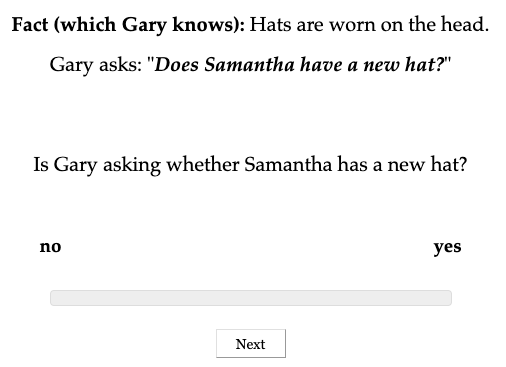
\includegraphics[height=5.4cm,width=7.6cm]{figures/exp1-nai-control}} 
\caption{Control trial in not-at-issueness block.}\label{fig-exp1-nai-control}
\end{subfigure}%
\begin{subfigure}[t]{0.5\textwidth}
\centering
\fbox{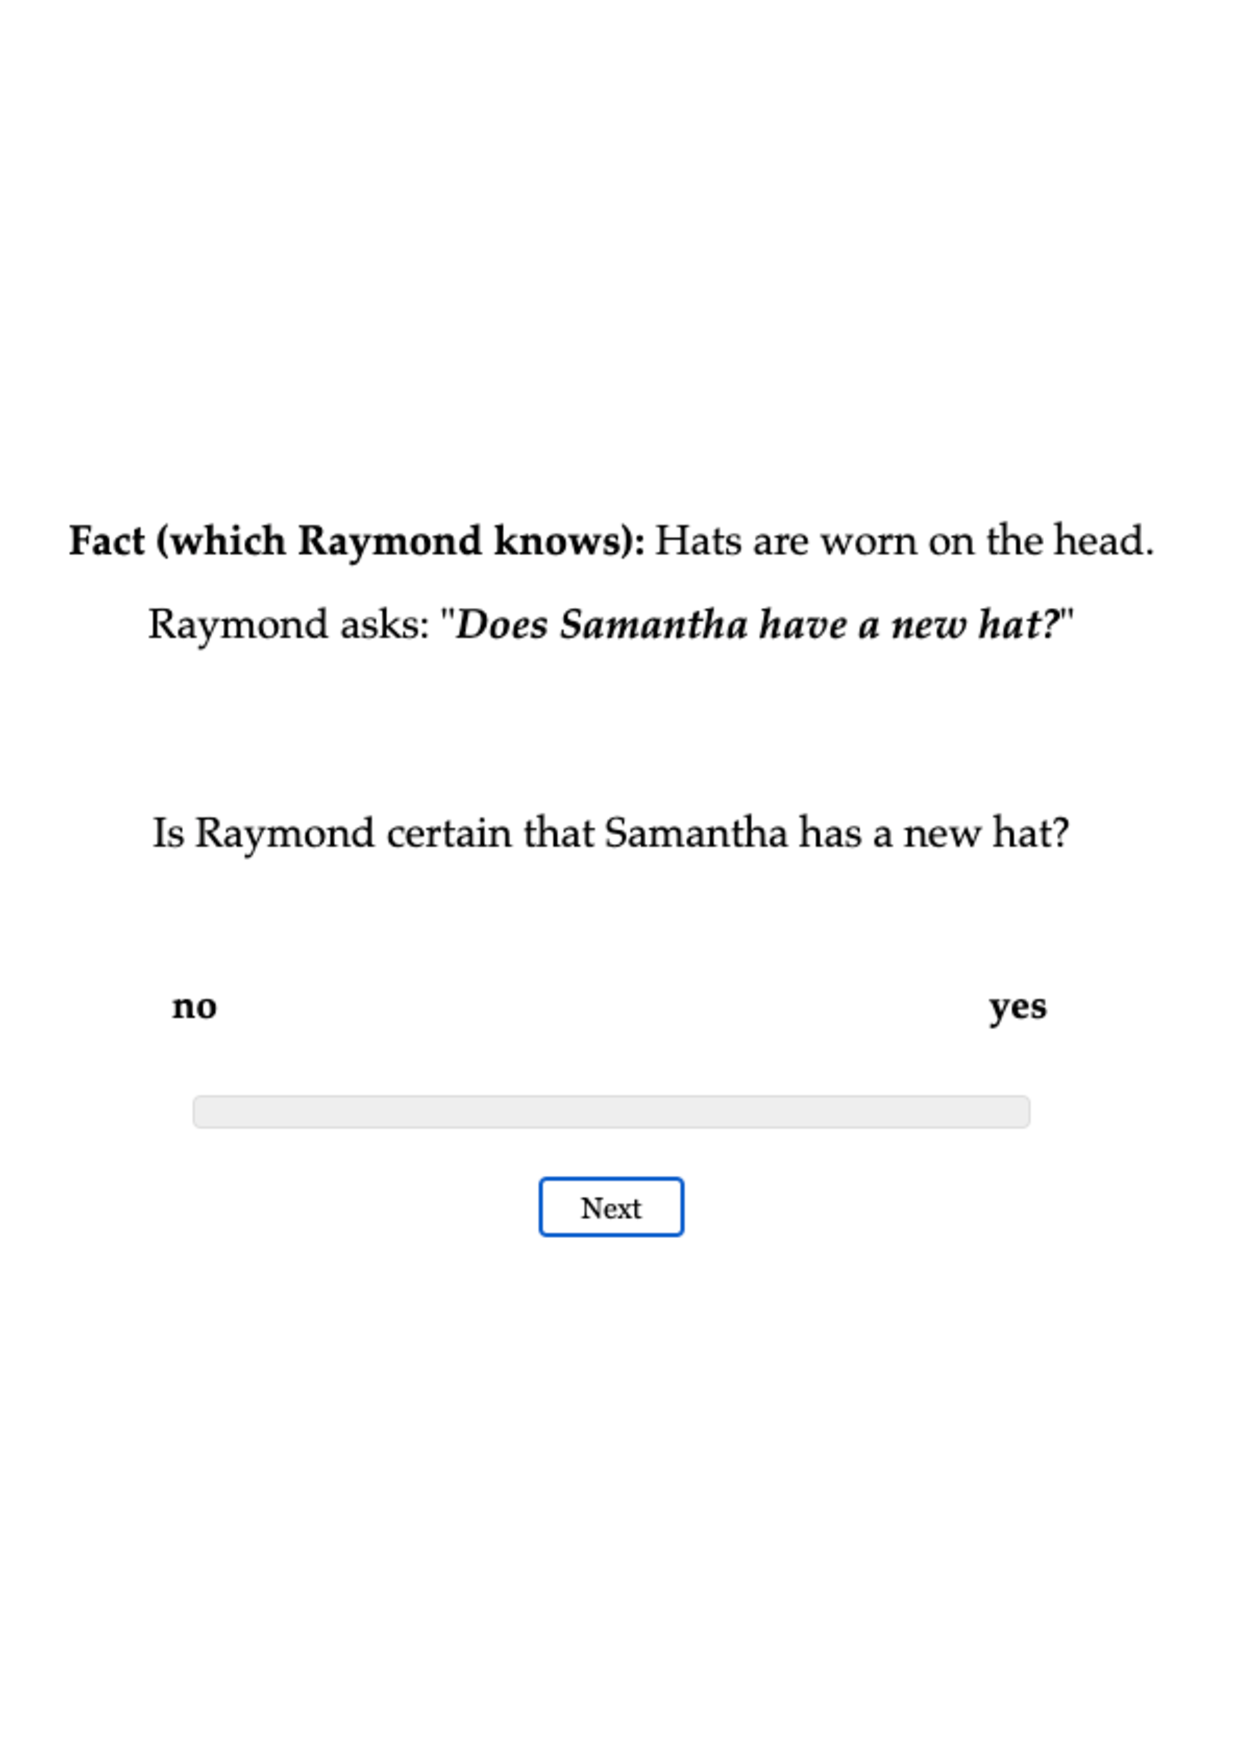
\includegraphics[height=5.4cm,width=7.6cm]{figures/exp1-projection-control}} 
\caption{Control trial in projection block.}\label{fig-exp1-projection-control}
\end{subfigure}

\caption{Sample control and filler trials in Exp.~1.}
\end{figure}

\begin{exe}
\ex\label{control-items}
\begin{xlist}
\ex Do these muffins have blueberries in them? Fact: Muffins are sold at the bakery. 
\ex Does this pizza have mushrooms on it? Fact: Pizza is sold at the pizzeria.
\ex Was Jack playing outside with the kids? Fact: Many children like ice cream.
\ex Does Ann dance ballet? Fact: Ballet is a type of dance.
\ex Were Carl's kids in the garage? Fact: Garages are used to store cars and other things.
\ex Does Samantha have a new hat? Fact: Hats are worn on the head.
\end{xlist}
\end{exe}

\section{Data exclusion}\label{a-excl}

We excluded the data from 16 participants who did not self-identify as native speakers of American English. We also excluded the data from one participant who always clicked on the same point of the scale across the target trials, as well as the data from 78 participants whose response means on the 6 not-at-issueness and projection control items were was more than 2 sd above the group means. Data from 505 participants (ages 20-73; mean age: 39.5) entered into the analysis (10,100 data points from target trials).

\section{Manipulation of prior beliefs}\label{a-beliefs}

%prior_type1 5.141e-01  9.979e-03 7.566e+02   51.52   <2e-16 ***

\figref{f-prior} shows the prior probability ratings of the 20 contents by fact. As shown, contents presented with the higher probability fact received higher prior probability ratings than contents presented with the lower probability fact. This result is confirmed by a mixed-effects linear regression model that predicts prior probability slider ratings from dummy-coded fact type (reference level: `lower probability') and random by-item and by-participant intercepts and slopes for fact type.  The content's mean prior probability was rated as higher when it was presented with its higher probability fact than when it was presented with its lower probability fact ($\beta$ = 0.51, $SE$ = 0.01, $t$ = 51.52, $p$ $<$ .0001). This result suggests that the manipulation of the prior probability of the 20 contents was successful. This result replicates the results of Exps.1 and 2a from \citealt{degen-tonhauser-openmind}.

\begin{figure}[h!]
\centering
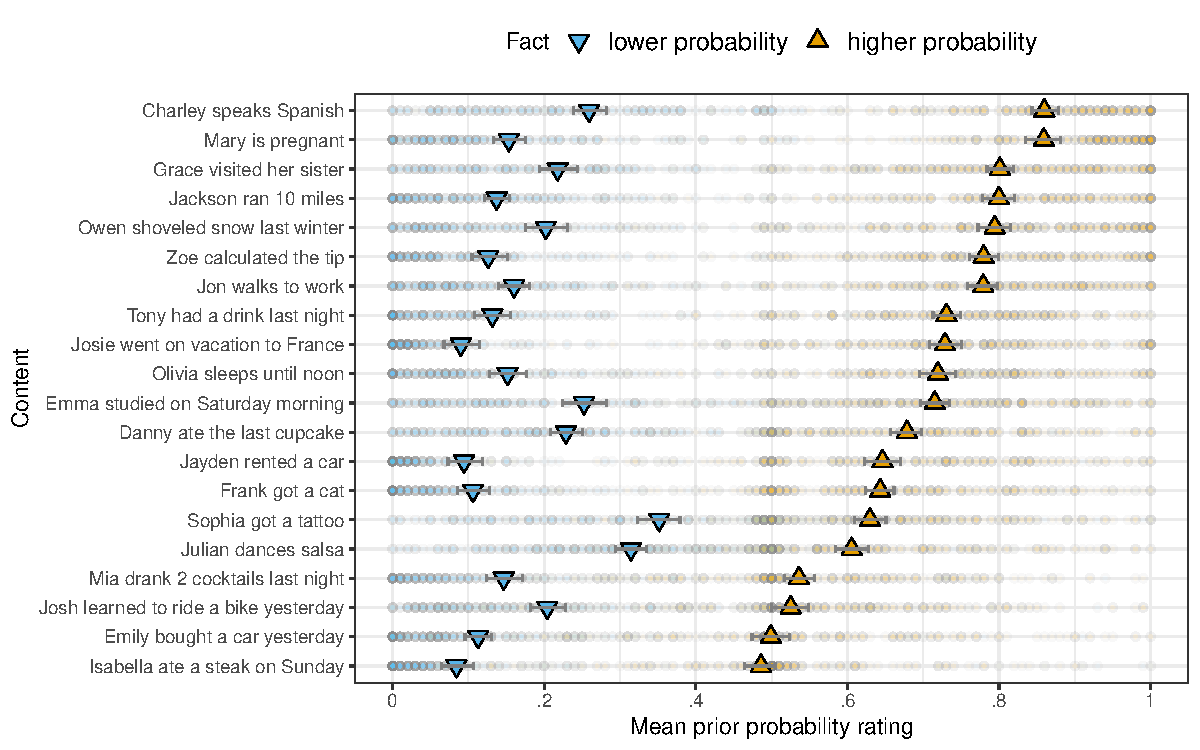
\includegraphics[width=.7\paperwidth]{../results/main/exp3/graphs/prior-ratings}

\caption{Mean prior probability rating by content and fact in Exp.~1. Error bars indicate 95\% bootstrapped confidence intervals. Transparent dots indicate individual participant ratings.} 
\label{f-prior}
\end{figure}


\section{Results of predicate interaction models}\label{a-models}

Table \ref{table:coefficients-prior} provides the details of the model predicting certainty ratings from prior probability ratings, predicate (with {\em be annoyed} as the reference level), and their interaction. Table \ref{table:coefficients-ai} provides the details of the model predicting certainty ratings from asking-whether ratings, predicate (with {\em be annoyed} as the reference level), and their interaction. 

\begin{table}
\begin{center}
\begin{tabular}{l r r l}
\toprule
Fixed effect & $\beta$ & {\em SE} & $p$-value \\ 
\midrule
(Intercept)                      &.83 & (.01) & $^{***}$  \\
prior prob.                           &.09 & (.04) & $^{*}$    \\
\midrule
inform             &-.12 & (.02) & $^{***}$ \\
acknowledge        &-.25 & (.02) & $^{***}$ \\
admit              &-.31 & (.02) & $^{***}$ \\
announce           &-.37 & (.02) & $^{***}$ \\
be right           &-.59 & (.02) & $^{***}$ \\
confess            &-.32 & (.02) & $^{***}$ \\
confirm            &-.54 & (.02) & $^{***}$ \\
demonstrate        &-.45 & (.02) & $^{***}$ \\
discover           &-.20 & (.02) & $^{***}$ \\
establish          &-.54 & (.02) & $^{***}$ \\
hear               &-.20 & (.02) & $^{***}$ \\
know               &-.06 & (.02) & $^{***}$ \\
pretend            &-.62 & (.02) & $^{***}$ \\
prove              &-.56 & (.02) & $^{***}$ \\
reveal             &-.28 & (.02) & $^{***}$ \\
say                &-.60 & (.02) & $^{***}$ \\
see                &-.15 & (.02) & $^{***}$ \\
suggest            &-.60 & (.02) & $^{***}$ \\
think              &-.59 & (.02) & $^{***}$ \\
\midrule
prior prob. $^*$ inform      &.01 & (.05)     \\
prior prob. $^*$ acknowledge &.12 & (.05) & $^{*}$    \\
prior prob. $^*$ admit       &.06 & (.05)     \\
prior prob. $^*$ announce    &.14 & (.05) & $^{**}$   \\
prior prob. $^*$ be right    &.12 & (.05) & $^{*}$    \\
prior prob. $^*$ confess     &.09 & (.05)     \\
prior prob. $^*$ confirm     &.08 & (.05)     \\
prior prob. $^*$ demonstrate &.13 & (.05) & $^{*}$    \\
prior prob. $^*$ discover    &.08 & (.05)     \\
prior prob. $^*$ establish   &.11 & (.05) & $^{*}$    \\
prior prob. $^*$ hear        &.11 & (.05) & $^{*}$    \\
prior prob. $^*$ know        &.03 & (.05)     \\
prior prob. $^*$ pretend     &.06 & (.05)     \\
prior prob. $^*$ prove       &.04 & (.05)     \\
prior prob. $^*$ reveal      &.05 & (.05)     \\
prior prob. $^*$ say         &.09 & (.05)     \\
prior prob. $^*$ see         &.10 & (.05) & $^{*}$    \\
prior prob. $^*$ suggest     &.09 & (.05)     \\
prior prob. $^*$ think       &.15 & (.05) & $^{**}$   \\
%\midrule
%AIC                              &2629.77$             \\
%BIC                              &2969.12$             \\
%Log Likelihood                   &-1267.88$            \\
%Num. obs.                        &10100$               \\
%Num. groups: workerid            &505$                 \\
%Num. groups: content             &20$                  \\
%Var: workerid (Intercept)        &.02$                 \\
%Var: workerid cprior             &.03$                 \\
%Cov: workerid (Intercept) cprior &-.00$                \\
%Var: content (Intercept)         &.00$                 \\
%Var: content cprior              &.00$                 \\
%Cov: content (Intercept) cprior  &.00$                 \\
%Var: Residual                    &.07$                 \\
\bottomrule
\multicolumn{2}{l}{\scriptsize{$^{***}p<0.001$; $^{**}p<0.01$; $^{*}p<0.05$}}
\end{tabular}
\caption{Details for model predicting certainty ratings from prior probability ratings, predicate (with {\em be annoyed} as the reference level), and their interaction.}
\label{table:coefficients-prior}
\end{center}
\end{table}

\begin{table}
\begin{center}
\begin{tabular}{l r r l}
\toprule
Fixed effect & $\beta$ & {\em SE} & $p$-value \\ 
\midrule %%%%%%%%% INSERT R OUTPUT STARTING HERE


(Intercept)                   & .27   & (.01) & $^{***}$  \\
not-at-issue                           & .06    & (.04) &        \\
\midrule
  be annoyed      & .43    & (.02) & $^{***}$  \\
  inform          & .37    & (.02) & $^{***}$  \\
  acknowledge     & .28    & (.02) & $^{***}$  \\
  admit           & .24    & (.02) & $^{***}$  \\
  announce        & .17    & (.02) & $^{***}$  \\
  be right        & .06    & (.02) & $^{*}$    \\
  confess         & .23    & (.02) & $^{***}$  \\
  confirm         & .06    & (.02) & $^{**}$   \\
  demonstrate     & .11    & (.02) & $^{***}$  \\
  discover        & .32    & (.02) & $^{***}$  \\
  establish       & .04    & (.02) & $^{*}$    \\
  hear            & .30    & (.02) & $^{***}$  \\
  know            & .41    & (.02) & $^{***}$  \\
  pretend         & -.03    & (.02) &       \\
  reveal          & .26    & (.02) & $^{***}$  \\
  say             & -.04    & (.02) & $^{*}$   \\
  see             & .36    & (.02) & $^{***}$  \\
  suggest         & -.05    & (.02) & $^{**}$  \\
  think           & -.04   & (.02) & $^{*}$   \\
\midrule
not-at-issue $^*$  be annoyed  & .38    & (.06) & $^{***}$  \\
not-at-issue $^*$  inform      & .31    & (.05) & $^{***}$  \\
not-at-issue $^*$  acknowledge & .24    & (.05) & $^{***}$  \\
not-at-issue $^*$  admit       & .17    & (.05) & $^{***}$  \\
not-at-issue $^*$  announce    & .12    & (.05) & $^{**}$   \\
not-at-issue $^*$  be right    & .16    & (.06) & $^{**}$   \\
not-at-issue $^*$  confess     & .11   & (.05) & $^{*}$    \\
not-at-issue $^*$  confirm     & .06    & (.05) &        \\
not-at-issue $^*$  demonstrate & .03    & (.05) &        \\
not-at-issue $^*$  discover    & .24    & (.05) & $^{***}$  \\
not-at-issue $^*$  establish   & -.00    & (.05) &       \\
not-at-issue $^*$  hear        & .29    & (.05) & $^{***}$  \\
not-at-issue $^*$  know        & .31    & (.05) & $^{***}$  \\
not-at-issue $^*$  pretend     & -.27    & (.05) & $^{***}$ \\
not-at-issue $^*$  reveal      & .17   & (.05) & $^{***}$  \\
not-at-issue $^*$  say         & -.05    & (.05) &       \\
not-at-issue $^*$  see         & .24    & (.05) & $^{***}$  \\
not-at-issue $^*$  suggest     & -.11    & (.05) & $^{*}$   \\
not-at-issue $^*$  think       & -.15    & (.05) & $^{***}$ \\
%\midrule
%AIC                           & $2273.51$             \\
%BIC                           & $2612.86$             \\
%Log Likelihood                & $-1089.75$            \\
%Num. obs.                     & $10100$               \\
%Num. groups: workerid         & $505$                 \\
%Num. groups: content          & $20$                  \\
%Var: workerid (Intercept)     & .01$                 \\
%Var: workerid not-at-issue $^*$             & .04$                 \\
%Cov: workerid (Intercept) not-at-issue $^*$ & $-.00$                \\
%Var: content (Intercept)      & .00$                 \\
%Var: content not-at-issue $^*$              & .00$                 \\
%Cov: content (Intercept) not-at-issue $^*$  & .00$                 \\
%Var: Residual                 & .06$                 \\

\bottomrule %%%%%%%%% END INSERTION OF R OUTPUT  HERE
\multicolumn{2}{l}{\scriptsize{$^{***}p<0.001$; $^{**}p<0.01$; $^{*}p<0.05$}}
\end{tabular}
\caption{Details for model predicting certainty ratings from asking-whether ratings, predicate (with {\em prove} as the reference level), and their interaction.}
\label{table:coefficients-ai}
\end{center}
\end{table}

\newpage

\section{Replication of by-predicate projection variation}\label{a-replication}

The mean certainty ratings of the predicates in the experiment reported  in this paper are compared in Fig.~\ref{fig:comparison-language} to those of Exp.~1 of \citealt{degen-tonhauser-language} (abbreviated `Exp 1 DT in print') and, in Fig.~\ref{fig:comparison-openmind}, to those of  Exp.~1 of \citealt{degen-tonhauser-openmind} (abbreviated `Exp 1 DT 2021'). 

\begin{figure}[h!]
\centering
\begin{subfigure}[t]{0.5\textwidth}
        \centering
\includegraphics[width=.3\paperwidth]{../results/main/exp3/graphs/projection-comparison-with-DT-Language}
\caption{}\label{fig:comparison-language}
 \end{subfigure}%
\begin{subfigure}[t]{0.5\textwidth}
\centering
\includegraphics[width=.3\paperwidth]{../results/main/exp3/graphs/projection-comparison-with-DT-OpenMind}
\caption{}\label{fig:comparison-openmind}
\end{subfigure}
\caption{Comparisons of mean by-predicate certainty ratings from the experiment reported on in this paper and Exp.~1 from \citealt{degen-tonhauser-openmind} (abbreviated `Exp 1 DT 2021'). Error bars indicate 95\% bootstrapped confidence intervals.} 
\label{f-comparison}
\end{figure}

\end{document}

